% =============================================================================================
% SECTION 3 -- RESULTS AND DISCUSSION.  Draft 2 -- merge of the former Sections 4, 5 and 6.
%
% Changes of substance from the split version:
%
%   * Every figure now has an introducing sentence in the body. Figs. 2, 4, 5 and 6 previously had
%     none -- Fig. 6 was reached only through another figure's caption, and Fig. 4(c) was never
%     referred to at all.
%   * Fig. 5 has moved to the subsection about the predictions it depicts; it used to sit fifty
%     lines inside the Refusals subsection.
%   * The Fig. 5 and Fig. 6 captions were carrying body content (Fig. 6's 175-word caption held
%     the only description of the conditional tier anywhere in the paper). That material is now in
%     the prose and the captions describe the figures.
%   * One funnel, not two. The 250/234 count and the 181/125 count are the same argument run over
%     two different candidate sets; the second was dropped and the first kept whole.
%   * The Ni-Sb member count is now stated with its set: 29.2 % is over the EIGHT in-domain
%     members, the Fig. 5 envelope is over TEN measured members. Both were correct and the
%     manuscript previously gave them without saying which was which.
%   * The refusal catalogue is a table; it was 600 words of prose.
%
% All labels from the split sections are preserved so existing \ref calls still resolve.
% =============================================================================================

\section{Results and Discussion}
\label{sec:results}

\subsection{Calculations exceed measurements, and the offset is regular}
\label{sec:offset}

Whether a correction is possible at all depends on the offset between calculation and experiment
being systematic rather than idiosyncratic, so we measure it first. For the \num{34} in-domain half
Heuslers carrying both a laboratory measurement and a published transport calculation, the
calculated lattice thermal conductivity exceeds the measured value by a median factor of
\num{1.55}. The excess is not scatter about agreement: it is one-sided, present in every bonding
family, and grows towards low temperature, which is the signature expected when extrinsic
scattering truncates long phonon mean free paths that the calculation allows to propagate freely.

Figure~\ref{fig:offset} shows the offset and its removal. Applying Eq.~\eqref{eq:transfer} with
$c=\num{0.51}$ and $p=\num{0.80}$ fitted over the whole domain---the constants a user of the method
would apply---brings the median ratio from \num{1.55} to \num{1.03}, and raises the fraction of
compound--temperature points within a factor of two of measurement from \SI{72}{\percent} to
\SI{87}{\percent}. The correction therefore centres the population, not merely shrinks it towards
the data. The accuracy figures below are scored under a stricter arrangement, with the
calibration refitted for each held-out chemistry; across those refits $c$ varies only between
\num{0.48} and \num{0.51}.

\begin{figure*}[tp]
  \centering
  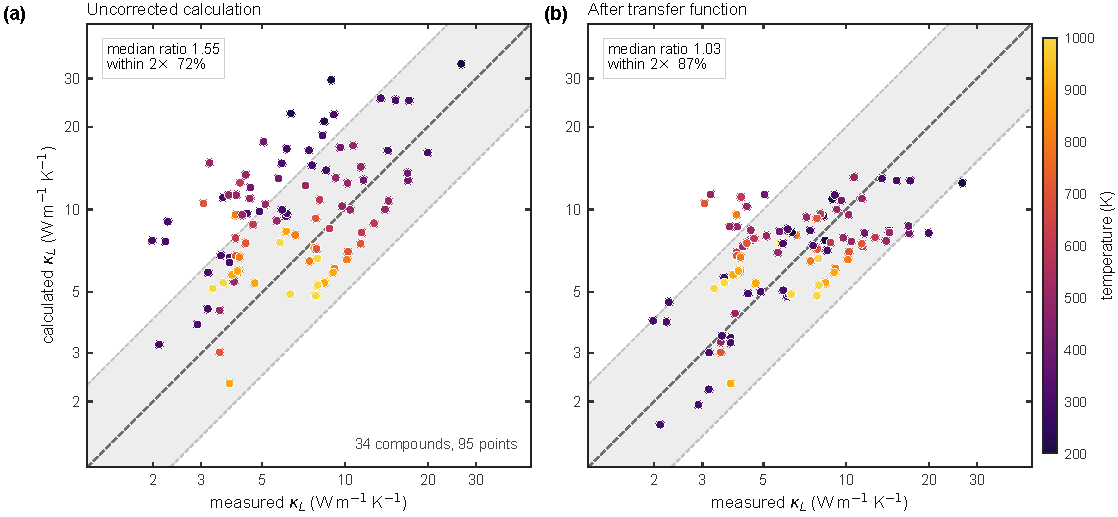
\includegraphics[width=\linewidth]{figures/fig02_offset.pdf}
  \caption{\textbf{Published transport calculations exceed laboratory measurements by a median
  factor of \num{1.55}; the transfer function removes the offset.}
  (a) Calculated against measured $\kappa_L$ for \num{34} in-domain half Heuslers,
  \num{95} compound--temperature points. (b) The same points after Eq.~\eqref{eq:transfer}.
  Shading marks a factor of two. Points are per compound per \SI{100}{\kelvin} bin, not per
  measurement row, since a few heavily sampled compounds (\ce{TiNiSn} \num{753} rows,
  \ce{ZrNiSn} \num{646}) would otherwise dominate.}
  \label{fig:offset}
\end{figure*}

\subsection{Blind-test accuracy}
\label{sec:blind}

Table~\ref{tab:blind} gives the central result. One thing about it should be said before the
numbers rather than after: the predictor being corrected here is the regression model of
Section~\ref{sec:model}, because that is the only one evaluable for all \num{38} compounds. The
route actually deployed for the predictions of Section~\ref{sec:issued} calibrates the
\emph{published} transport calculation instead, and it is more accurate---\SI{27.3}{\percent}
against \SI{31.4}{\percent}, scored separately in Section~\ref{sec:deployed}. Table~\ref{tab:blind}
is therefore the conservative of the two routes.

Across \num{38} half Heuslers spanning \num{18}
chemistry clusters, each predicted with its entire chemistry removed from training, the calibrated
prediction achieves a median absolute error of \SI{33.7}{\percent}---the median over five model
seeds, which individually range from \SI{31.0}{\percent} to \SI{40.0}{\percent}---and places
\SI{86.8}{\percent} of compounds within a factor of two of the measurement. The same model output
without the correction gives \SI{50.5}{\percent} and \SI{65.8}{\percent}. The median ratio of
predicted to measured conductivity is \num{1.00}, against \num{1.32} uncorrected, so the method is
centred and not merely closer. Under the tighter criterion
of \SI{30}{\percent}, the fraction rises from \SI{21.1}{\percent} to \SI{42.1}{\percent}, so two
compounds in five are predicted to within a third.

\begin{table*}[tp]
  \centering
  \caption{Blind-test performance inside the declared domain of applicability. Every compound is
  predicted with its entire chemistry cluster withheld from training, and all nulls are fitted with
  the same chemistry held out as the calibration. Rows that depend on the regression model---the
  first two and the one-parameter ablation---are medians over five model seeds; the nulls, the
  family baseline and the semi-empirical estimates do not depend on the model and are single
  values.}
  \label{tab:blind}
  \begin{tabular}{lcccc}
    \toprule
    & median error & within $2\times$ & within \SI{30}{\percent} & bias \\
    \midrule
    Calibrated (this work)   & \textbf{\SI{33.7}{\percent}} & \textbf{\SI{86.8}{\percent}}
                             & \textbf{\SI{42.1}{\percent}} & \textbf{1.00} \\
    Uncorrected surrogate    & \SI{50.5}{\percent} & \SI{65.8}{\percent}
                             & \SI{21.1}{\percent} & 1.32 \\
    Null: constant $\kappa$  & \SI{44.0}{\percent} & \SI{78.9}{\percent}
                             & \SI{26.3}{\percent} & 1.20 \\
    Null: $A(T/300)^{q}$     & \SI{44.9}{\percent} & \SI{81.6}{\percent}
                             & \SI{26.3}{\percent} & 1.17 \\
    \midrule
    Null: family power law$^{\ddagger}$ & \SI{28.2}{\percent} & \SI{87.1}{\percent}
                             & --- & 1.01 \\
    \midrule
    One parameter, $c$ only  & \SI{44.3}{\percent} & \SI{68.4}{\percent} & \SI{31.6}{\percent} & 0.96 \\
    Slack / Debye--Callaway$^{\dagger}$ & \SI{94.6}{\percent} & \SI{52.4}{\percent} & --- & 1.95 \\
    \bottomrule
    \multicolumn{5}{l}{\footnotesize $^{\dagger}$ published semi-empirical estimates, on the
      \num{21} in-domain compounds that carry one.} \\
    \multicolumn{5}{l}{\footnotesize $^{\ddagger}$ on the \num{31} compounds whose bonding family
      has $\geq 2$ other measured members; see Section~\ref{sec:familynull}.}
  \end{tabular}
\end{table*}

Figure~\ref{fig:curves} shows what this means for individual compounds. Nine are drawn at the
tercile boundaries of the error distribution---the three best, three central and three worst of the
\num{28} in-domain compounds with at least five measured temperatures spanning
\SI{300}{\kelvin}---so the selection is arithmetic rather than editorial. Their median error
(\SI{35.8}{\percent}) matches that of all \num{28} (\SI{33.6}{\percent}), but by construction they
over-represent the tails: their interquartile range is \SI{79}{\percent} against \SI{30}{\percent}
for the full set. The figure is therefore a fair sample of the centre and a deliberately pessimistic
one of the spread. It also shows plainly what the method does not deliver. The predicted curves are
visibly flatter than the measurements in several panels, because Eq.~\eqref{eq:transfer} carries a
single global exponent; the magnitude is corrected, the shape is not.

\begin{figure*}[tp]
  \centering
  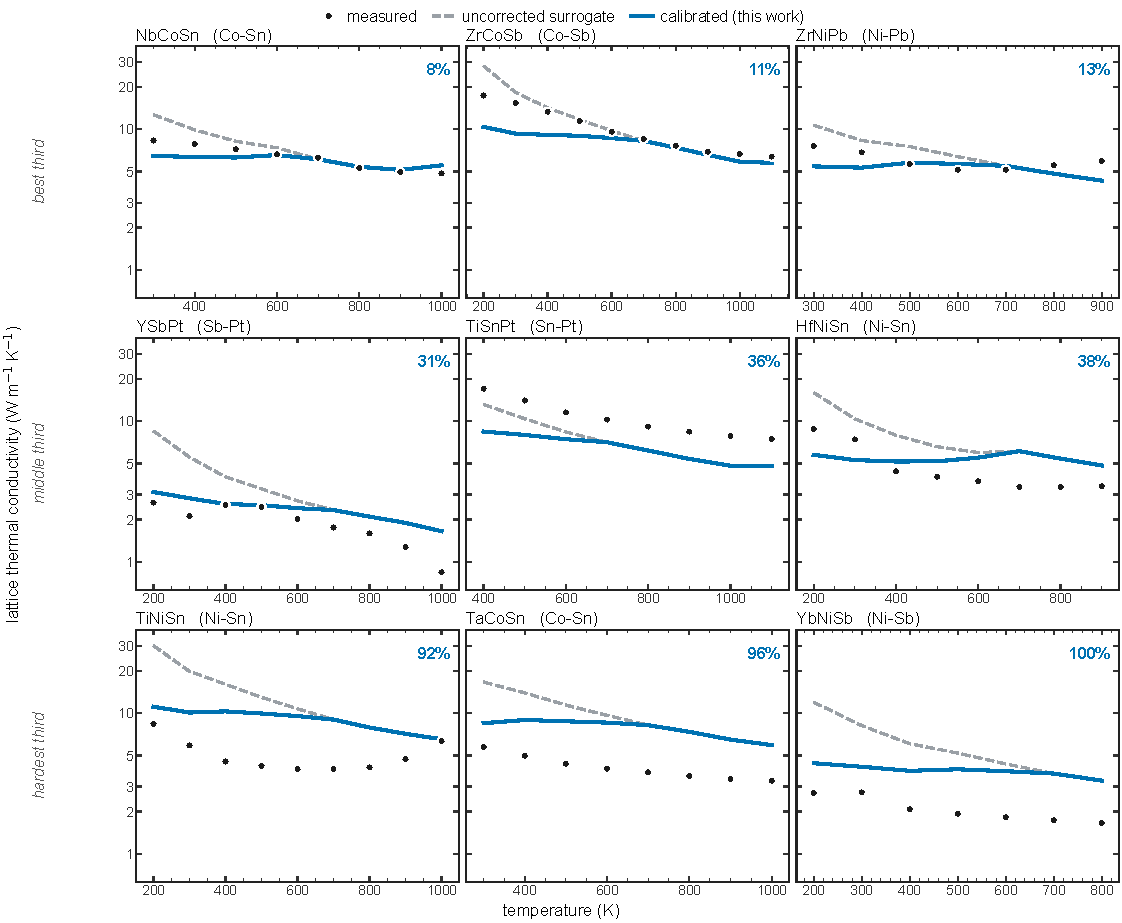
\includegraphics[width=\linewidth]{figures/fig03_curves.pdf}
  \caption{\textbf{The calibrated prediction lands on the measured magnitude; the temperature
  slope is not predicted.} Measured $\kappa_L(T)$ (points), the uncorrected \emph{surrogate}
  (dashed) and the calibrated prediction (solid) for nine in-domain compounds, each with its
  chemistry held out of both the surrogate and the calibration. The dashed curve is the regression
  model's output, not a published transport calculation: the two differ by a median
  \SI{15.4}{\percent} and are scored separately in Section~\ref{sec:deployed}. Rows are the best,
  middle and hardest thirds of the error distribution, drawn at the tercile boundaries;
  per-compound median error is given in each panel.}
  \label{fig:curves}
\end{figure*}

\subsection{Comparison with baselines}
\label{sec:vsnulls}
\label{sec:baselines}

A prediction of $\kappa_L$ earns nothing unless it beats predictors that use no compound-specific
information. Against the two compound-blind nulls of Section~\ref{sec:nulls}, both refitted with
the same chemistry held out as the calibration, the calibrated prediction is better on every metric
in Table~\ref{tab:blind} and closer to the measurement for \SI{65.8}{\percent} of compounds. A paired
Wilcoxon signed-rank test over per-compound errors gives $p=\num{0.050}$ against the constant null
and $p=\num{0.048}$ against the power law, taking the median over seeds; three of the five seeds
clear both nulls at \num{0.05} and two do not. Two qualifications belong with those figures. Both
$p$-values sit at the conventional threshold and would be marginal under a strict correction for
two comparisons, so we present them as evidence rather than proof. And the same test computed over
all \num{51} half Heuslers, before the domain screens are applied, gives $p=\num{0.30}$ and
$p=\num{0.72}$: the separation appears only once the domain is imposed. We regard that as the
expected consequence of removing thirteen compounds in which lattice conduction is not the dominant
channel, and note that the screens were fixed before the validation set was scored. Both numbers
are given.

The rank correlation is the more robust claim---Spearman's
$\rho$ between predicted and measured conductivity is \num{0.65} across the \num{38} compounds
(seed range \numrange{0.618}{0.675}, $p<\num{1e-4}$ for every seed)---and ordering candidates
reliably is what a screening application requires.

Two further comparisons test the method against something better than a null. Both are ablations run
at a single fixed model seed, at which the method's reference figure is \SI{31.0}{\percent} rather
than the seed-median \SI{33.7}{\percent}. Semi-empirical Slack and Debye--Callaway models are the standard cheap route to
$\kappa_L$, and \num{21} of our in-domain compounds carry such an estimate in the literature. On
those \num{21} the published estimates give a median error of \SI{94.6}{\percent} with a bias of
\num{1.95}, against \SI{31.5}{\percent} for the calibrated calculation on the same compounds
(paired Wilcoxon $p=\num{2e-4}$, ours closer for \SI{81}{\percent} of them); no holdout is applied
to the semi-empirical values, which if anything favours them. Dropping our own temperature exponent,
so that $\kappa_L^{\mathrm{expt}} = c\,\kappa_L^{\mathrm{BTE}}$ with a single fitted constant,
raises the median error from \SI{31.0}{\percent} to \SI{45.1}{\percent} and drops the
within-$2\times$ fraction from \SI{86.8}{\percent} to \SI{71.1}{\percent} ($p=\num{0.001}$).
Averaged over seeds the gap is \SI{33.7}{\percent} against \SI{44.3}{\percent}. The exponent is
doing real work, and the method is not a single scale factor with decoration.

\subsection{A stronger baseline: the compound's own bonding family}
\label{sec:familynull}

The nulls above are compound-blind by construction, and the obvious informed alternative is to fit
a power law to the \emph{measured} $\kappa(T)$ of the held-out compound's own
$(\mathrm{Y},\mathrm{Z})$ bonding family and use that. It needs no first-principles calculation, no
regression model and no calibration. It is a strong baseline, and we report it as such: fitted
leave-one-chemistry-out like everything else, it achieves \SI{28.2}{\percent} median error on the
\num{31} in-domain compounds whose family has at least two other measured members
(Table~\ref{tab:populations}). Scored on those same \num{31} our method gives \SI{33.3}{\percent};
the \SI{31.0}{\percent} quoted elsewhere is over all \num{38}, and comparing the two would
understate the gap. Head to
head the difference is not significant (paired Wilcoxon $p=\num{0.22}$) and our method is the closer
of the two for only \SI{42}{\percent} of them. \textbf{On absolute accuracy we do not beat it.}

Two things nonetheless separate the two, and both bear on how the predictions below should be read.
The first is coverage: the family baseline is undefined for \num{7} of the \num{38} in-domain
compounds (\ce{AlVNi}, \ce{NbFeSb}, \ce{TaFeSb}, \ce{YNiBi}, \ce{ZrCoBi}, \ce{ZrNiPb},
\ce{ZrSbIr}), whose families hold too few measured members, whereas a calibrated calculation is
available wherever a calculation is. The second is more fundamental. A family power law returns one
curve per family, so every member receives essentially the same prediction---across our families
the spread between members is only \numrange{1.1}{1.8}---and it therefore cannot order compounds
within a family. Measured against the true ordering, the within-family Spearman correlation is
$-0.90$ for the family baseline and $+0.50$ for the calibrated calculation; in the two families
where we issue predictions the gap is starkest, $+0.93$ against $-0.67$ for \ce{Ni}--\ce{Sb}
($n=8$) and $+0.60$ against $-1.00$ for \ce{Sb}--\ce{Pt} ($n=4$). These correlations rest on three
to eight compounds each and are indicative rather than precise. But within-family ranking is
exactly the task a screening user faces---choosing between \ce{ErSbPt}, \ce{HoSbPt} and
\ce{TmSbPt}, three members of one substitution series, is a within-family problem---and the family
baseline is uninformative for it by construction. The contribution of the calibrated calculation is
not that it predicts the family level better, but that it resolves structure inside a family that a
family-level baseline cannot see.

\subsection{The route that is actually deployed}
\label{sec:deployed}

Table~\ref{tab:blind} is computed on the regression model's output, because that is the predictor
which can be evaluated for all \num{38} compounds. It is not the published transport value: the two
differ by a median of \SI{15.4}{\percent}, and the predictions of Section~\ref{sec:issued} are
issued by calibrating the \emph{published} calculation. That route deserves to be scored on its
own. On the \num{34} in-domain compounds carrying a temperature-matched published transport value,
the uncorrected published calculation gives \SI{71.6}{\percent} median error at a bias of \num{1.72}
and the uncorrected surrogate \SI{66.1}{\percent} at \num{1.66}; calibrated, the surrogate gives
\SI{31.4}{\percent} at \num{1.05} and the published calculation \SI{27.3}{\percent} at \num{1.09}.
The bias of \num{1.72} here and the factor of \num{1.55} quoted in Section~\ref{sec:offset} are the
same offset aggregated two ways: \num{1.55} is the median over the \num{95} compound--temperature
bins of Fig.~\ref{fig:offset}, \num{1.72} the median over the \num{34} compounds. We quote the
binned figure when describing the offset because it is what the figure shows, and the per-compound
figure whenever a compound-level error is being scored.
Two things follow. The uncorrected published calculation is \emph{worse} than the uncorrected
surrogate, so the improvement the transfer function delivers over a raw first-principles value is
larger than Table~\ref{tab:blind} implies, not smaller. And the route we deploy is the better of the
two: where a transport calculation exists, it should be calibrated directly rather than replaced by
a model.

\subsection{Where the method fails, and what did not fix it}
\label{sec:failure}
\label{sec:rejected}

Two failure modes are visible, and both are identifiable in advance. Outside the declared domain
the thirteen excluded compounds have a median error of \SI{105.1}{\percent} against
\SI{29.7}{\percent} inside it, both scored under the single calibration a user would apply
(Mann--Whitney $p=\num{7.5e-3}$); their uncorrected calculations are also far worse and they require
a quite different calibration constant, so they are a distinct population rather than merely harder
examples. Inside the domain, failure sorts by bonding family. Figure~\ref{fig:blind} shows both
effects together with the comparison against the nulls. Grouping in-domain compounds by their
$(\mathrm{Y},\mathrm{Z})$ site pair---the two more electronegative sites, which form the covalent
sublattice that carries the heat---separates the accurate families from the inaccurate:
\ce{Co}--\ce{Sb} (\SI{21.3}{\percent}), \ce{Sb}--\ce{Pt} (\SI{23.2}{\percent}) and
\ce{Ni}--\ce{Sb} (\SI{29.2}{\percent}) are predicted well, while \ce{Co}--\ce{Sn}
(\SI{80.8}{\percent}) and \ce{Bi}--\ce{Pd} (\SI{60.0}{\percent}) are not. The two fail differently,
and the difference decides what we do about them. Every \ce{Co}--\ce{Sn} member still lands within a
factor of two, so its predictions stay inside the band this method claims. \ce{Bi}--\ce{Pd} does
not: only \SI{33}{\percent} of its members are within a factor of two, and its median bias of
\num{0.40} is a systematic \num{2.5}-fold under-prediction rather than scatter. We issue no
predictions in either family. Both rest on three compounds, so these figures indicate where to be
careful rather than measure a failure rate. This grouping is a \emph{post hoc} description of where errors
concentrate: the holdout unit throughout is the X site, not the $(\mathrm{Y},\mathrm{Z})$ pair, so
family members remain in training when a compound is held out and the family error is an
interpolation figure rather than an extrapolation test.

\begin{figure*}[tp]
  \centering
  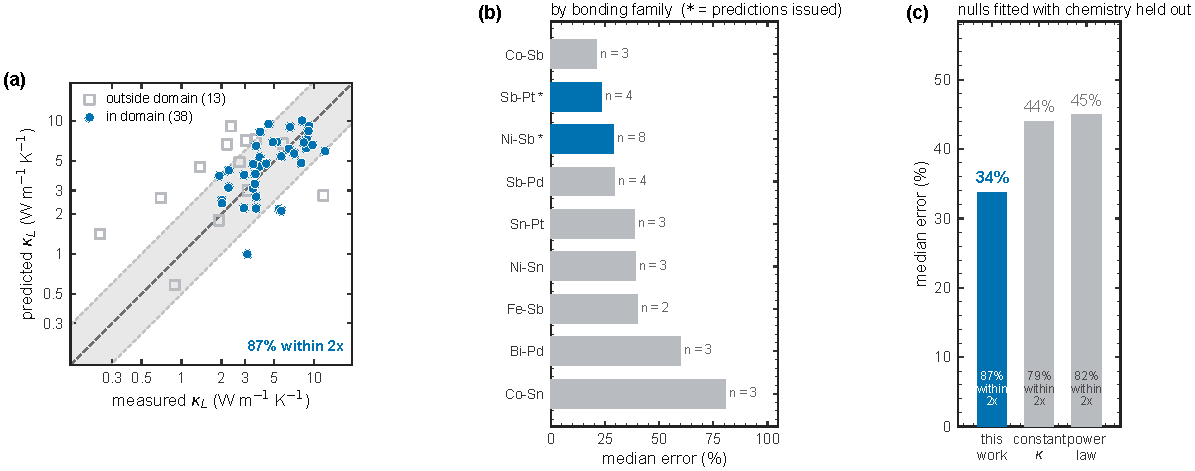
\includegraphics[width=\linewidth]{figures/fig04_blind.pdf}
  \caption{\textbf{\SI{86.8}{\percent} of in-domain compounds are predicted within a factor of
  two.} (a) Predicted against measured $\kappa_L$; open symbols are the thirteen compounds outside
  the declared domain, shown on the same axes. (b) Median error by $(\mathrm{Y},\mathrm{Z})$
  bonding family; starred families are those in which predictions are issued. (c) Against two
  compound-blind nulls, each fitted with chemistry held out; the bar for this work is the
  five-seed median of Table~\ref{tab:blind}, whereas panels (a) and (b) are necessarily drawn from
  a single seed.}
  \label{fig:blind}
\end{figure*}

Five modifications intended to repair these failures were implemented and evaluated under the same
protocol, and none survived it. A hurdle model treating low- and high-conductivity compounds
separately halves the low-$\kappa$ error on calculated labels but changes experimental accuracy by
\SI{-1.3}{pp} ($p=\num{0.84}$). A magnitude term $\kappa^{\beta}$ added to Eq.~\eqref{eq:transfer}
was selected on the design half in 47 of 60 splits and lost on the held-out half. Adding
experimental values to the training set gives \SI{+5.5}{pp} at $p=\num{0.10}$ and is worse on the
transition-metal subset; adding doped-composition data gives no gain at all ($p\geq\num{0.10}$).
Per-family calibration constants are the most interesting failure: the families genuinely do differ
in their raw calculation-to-measurement ratio, but the difference does not transfer, and under
leave-one-chemistry-out a per-family fit gives \SI{31.1}{\percent} against \SI{31.0}{\percent} for
the single global constant ($p=\num{0.22}$, better for only 17 of \num{38} compounds). With two to
four measured members per family, the apparent differences are noise. The single global transfer
function therefore remains the reported method.

\subsection{Predictions for unmeasured compounds}
\label{sec:predictions}
\label{sec:screening}
\label{sec:issued}

We now apply the method to half Heuslers that carry a published transport calculation but no
laboratory measurement, calibrating that published calculation directly. A candidate is carried
forward only if it satisfies every condition below, all evaluated in code at the point the
prediction list is generated, so a compound that fails one cannot reappear in a later regeneration:

\begin{enumerate}
  \item The three domain conditions of Section~\ref{sec:domain}.
  \item \textbf{Not polymorphic.} Which phase forms on synthesis is not ours to assume.
  \item \label{itm:family} \textbf{A validated bonding family:} the $(\mathrm{Y},\mathrm{Z})$
        family must contain at least two compounds predicted correctly against measurement.
        \ce{Bi}--\ce{Pd} is excluded outright on the evidence of Section~\ref{sec:failure}.
  \item \textbf{The label is a transport calculation}, matched on the method string.
  \item \textbf{Inside the family's measured range.} A prediction falling outside the span its own
        family has been measured in is an extrapolation, and is flagged as one rather than issued.
\end{enumerate}

Condition~\ref{itm:family} removes more candidates than the other four together, so it deserves the
most scrutiny. We evaluated it leave-one-out across the \num{36} in-domain compounds for which a
measurement exists, counting the usable anchors in each compound's family \emph{excluding the
compound itself}, which is the situation an unmeasured target actually faces. Compounds whose family
then holds two or more anchors have a median error of \SI{32.3}{\percent} with \SI{96.2}{\percent}
inside a factor of two ($n=\num{26}$); those whose family holds none reach \SI{37.2}{\percent} with
\SI{75}{\percent} inside ($n=\num{8}$). The remaining \num{2} hold exactly one anchor and are the
subject of the relaxation test below. The separation is carried by the within-$2\times$ rate
rather than by the median, and we state it no more strongly than that. Relaxing the threshold from
two anchors to one fails: the two compounds the weaker rule admits have a median error of
\SI{45.5}{\percent} against \SI{32.3}{\percent}. The intuitive alternative---requiring many
chemically similar training compounds---does not survive testing either, since ranking those same
\num{36} compounds by how many calculated compounds share their X site gives a Spearman correlation
with error of $+\num{0.044}$ ($p=\num{0.80}$). What makes a prediction trustworthy here is not the
volume of nearby chemistry but whether an answer has ever been checked in that family.

Five candidates satisfy all five conditions, and they are the complete set rather than a selection.
Enumerating every half Heusler in the corpus that carries a genuine transport calculation between
\SI{150}{\kelvin} and \SI{450}{\kelvin} and has no measurement of its own gives \num{181} compounds,
of which \num{125} clear scope, $\mathrm{VEC}=18$, a cubic record and the radioactivity screen. The
family condition then eliminates almost all the remainder: \num{97} sit in a family with no usable
measured member, \num{9} are \ce{Bi}--\ce{Pd}, \num{8} carry independent calculations that disagree
by a factor of two or more, and \num{1} sits in a family one measurement short. Exactly \num{10}
sit in a validated family, and they are precisely the five predictions and the five flagged cases
below. The binding constraint is therefore not chemistry, not structure and not the availability of
calculations, but the absence of measurements in the families concerned.

Table~\ref{tab:predictions} gives the five, and Fig.~\ref{fig:predictions} draws them inside the
measurements that license them. The transport calculations being calibrated are not ours: they come
from published high-throughput
studies~\cite{li2025highthroug,ohnishi2026database,miyazaki2021machine}, and each predicted value is
that published number multiplied by the transfer function. \ce{ErSbPt} and \ce{HoSbPt} rest on
\num{85} calculated rows each, \ce{TmSbPt}, \ce{GdNiSb} and \ce{TbNiSb} on two or three. The two
families involved are the best predicted in the blind test after \ce{Co}--\ce{Sb}: \ce{Sb}--\ce{Pt}
at \SI{23.2}{\percent} median error over its four in-domain measured members and \ce{Ni}--\ce{Sb} at
\SI{29.2}{\percent} over its eight. Every predicted value falls inside the measured span of its own
family---\SIrange{2.1}{3.8}{\watt\per\meter\per\kelvin} for \ce{Sb}--\ce{Pt} and
\SIrange{2.3}{14.5}{} for \ce{Ni}--\ce{Sb}---so none requires the method to extrapolate beyond
conductivities experiment has already reached in that chemistry. Three of the five (\ce{ErSbPt},
\ce{HoSbPt}, \ce{TmSbPt}) come from a single substitution series in which only the rare-earth site
varies, so the covalent \ce{Sb}--\ce{Pt} sublattice that carries the heat is common to all three and
to the measured members; \ce{GdNiSb} and \ce{TbNiSb} stand in the same relation to the measured
\ce{Ni}--\ce{Sb} compounds. One restriction applies to how they are read: \ce{TmSbPt}, \ce{GdNiSb}
and \ce{TbNiSb} rest on a single calculated temperature, so their values at \SI{600}{\kelvin} and
\SI{900}{\kelvin} would carry only the global exponent and no compound-specific temperature
dependence, and are not quoted. Only \ce{ErSbPt} and \ce{HoSbPt} support a curve.

\begin{table*}[tp]
  \centering
  \caption{Predicted lattice thermal conductivity at \SI{300}{\kelvin} for half Heuslers with a
  published transport calculation and no measurement. All five fall inside the range their own
  bonding family has been measured in, so each is an interpolation within validated chemistry.
  Intervals are conformal (Section~\ref{sec:intervals}).}
  \label{tab:predictions}
  \begin{tabular}{llcccc}
    \toprule
    Compound & Family & $\kappa_L^{\mathrm{BTE}}$ & \textbf{Predicted} &
      \SI{50}{\percent} interval & \SI{90}{\percent} interval \\
    & & \multicolumn{4}{c}{(\si{\watt\per\meter\per\kelvin})} \\
    \midrule
    \ce{TmSbPt} & \ce{Sb}--\ce{Pt} & 5.86 & \textbf{2.99} & 2.28--3.92 & 1.33--6.70 \\
    \ce{HoSbPt} & \ce{Sb}--\ce{Pt} & 7.00 & \textbf{3.57} & 2.73--4.68 & 1.59--8.00 \\
    \ce{ErSbPt} & \ce{Sb}--\ce{Pt} & 7.18 & \textbf{3.66} & 2.79--4.79 & 1.63--8.20 \\
    \ce{GdNiSb} & \ce{Ni}--\ce{Sb} & 8.38 & \textbf{4.27} & 3.26--5.59 & 1.91--9.56 \\
    \ce{TbNiSb} & \ce{Ni}--\ce{Sb} & 9.06 & \textbf{4.62} & 3.53--6.05 & 2.06--10.35 \\
    \bottomrule
  \end{tabular}
\end{table*}

\begin{figure*}[tp]
  \centering
  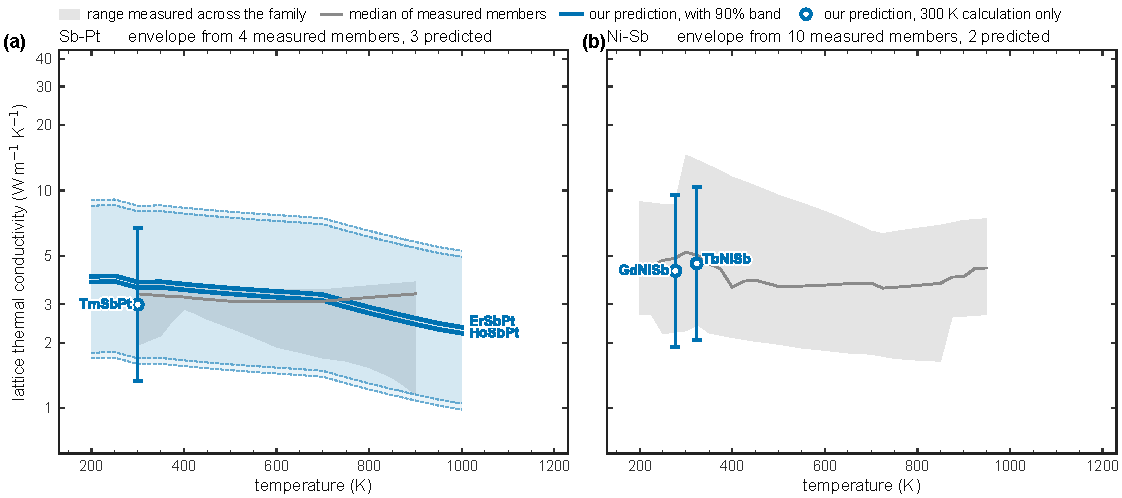
\includegraphics[width=\linewidth]{figures/fig05_predictions.pdf}
  \caption{\textbf{The five issued predictions, drawn inside the measurements that license
  them.} For each validated bonding family the range spanned by that family's measured members is
  shaded, with their median as a grey line, and the predicted compounds are drawn over it in blue
  with their \SI{90}{\percent} conformal band. (a)~\ce{Sb}--\ce{Pt}: envelope from four measured
  members, three predictions. (b)~\ce{Ni}--\ce{Sb}: envelope from ten measured members, two
  predictions. The envelope is drawn over every measured member of the family; the family error
  quoted in the text is over in-domain members only, of which \ce{Ni}--\ce{Sb} has eight.
  \ce{TmSbPt}, \ce{GdNiSb} and \ce{TbNiSb} have a single calculated value at \SI{300}{\kelvin} and
  are drawn as points with their interval; where two coincide their horizontal separation is
  cosmetic. The ordinate is logarithmic because the transfer function is multiplicative.}
  \label{fig:predictions}
\end{figure*}

\subsection{Candidates we decline, and the measurement that would qualify them}
\label{sec:refusals}
\label{sec:whyfive}
\label{sec:novel}

Eleven candidates are declined, and the reasons are as much a result as the five predictions.
Table~\ref{tab:refusals} names them with the condition each fails. Five are flagged---a value
exists and a named check fails---while six are refused outright, and for those six the calibrated
number is not a quantity we are willing to give. The four flagged for falling outside their family's
measured range are not equivalent cases, as the table's margins show: \ce{LaSbPt} and \ce{ScSbPt}
are clear extrapolations, whereas \ce{TmSbPd} and \ce{GdSbPt} miss by less than the factor of
\num{1.33} by which laboratories measuring the same compound routinely disagree. We hold the last
two back as a stated conservatism rather than a validated filter. The boundary is a min--max over
three to five measured compounds and would move if one more were measured, and applied
retrospectively to the \num{16} measured compounds whose families are large enough to test it, the
rule does not separate good predictions from bad (\SI{29.6}{\percent} against \SI{24.8}{\percent},
$p=\num{0.35}$). We keep it because withholding a prediction costs nothing and issuing a wrong one
costs a synthesis, but a reader who weighs that differently has the margins.

\begin{table*}[tp]
  \centering
  \caption{The eleven declined candidates and the condition each fails. Flagged compounds have a
  calibrated value that we do not issue; refused compounds are ones for which we decline to compute
  one.}
  \label{tab:refusals}
  % The third column holds full sentences, so it needs an explicit width. Left as `l' it sets on a
  % single line and runs past the right margin, which is what overlapped the following paragraph.
  \begin{tabular}{llp{0.52\linewidth}}
    \toprule
    Compound & Status & Condition failed \\
    \midrule
    \ce{DySbPd} & flagged  & polymorphic: space group 216 recorded alongside 186 and 194 \\
    \ce{LaSbPt} & flagged  & \num{2.39} below the measured \ce{Sb}--\ce{Pt} floor \\
    \ce{ScSbPt} & flagged  & \num{1.65} above the measured \ce{Sb}--\ce{Pt} ceiling \\
    \ce{GdSbPt} & flagged  & \num{1.24} beyond the nearest measured edge \\
    \ce{TmSbPd} & flagged  & \num{1.09} beyond the nearest measured edge \\
    \midrule
    \ce{TiNiSb} & refused  & $\mathrm{VEC}\neq 18$ \\
    \ce{CrSnPt} & refused  & $\mathrm{VEC}\neq 18$ \\
    \ce{ThNiSn} & refused  & thorium: no training example in the corpus \\
    \ce{ThSnPt} & refused  & thorium: no training example in the corpus \\
    \ce{UNiSn}  & refused  & uranium: no training example in the corpus \\
    \ce{USnPt}  & refused  & uranium: no training example in the corpus \\
    \bottomrule
  \end{tabular}
\end{table*}

Five predictions from a corpus of \num{742} half Heuslers invites the question of where the rest
went, and the answer is not a limitation of the method but a statement about the experimental
literature. Figure~\ref{fig:landscape} sets out everything the method can say and what each
statement is worth, in four tiers. Below the five issued and the eleven declined sits a third tier
of \num{10} compounds that pass every structural and chemical screen but sit in a family with no
usable measured anchor---nine of them \ce{Ni}--\ce{Bi}. These are conditional: the method would
predict them the moment their family acquired two sound measurements, and they are tabulated with
the measurement each waits on in Table~S1 of the supplementary material. Their existence makes the
binding constraint concrete: five laboratory measurements across four bonding families would take
the method from five predictions to nineteen, of which fourteen survive every screen that does not
depend on the new measurement. The ten conditional estimates of Table~S1 are the subset of those
fourteen that carry a calculation at room temperature and can therefore be quoted with a value; the
other four have a transport calculation but not one at \SI{300}{\kelvin}. \ce{Ni}--\ce{Bi} is the most economical, releasing nine predictions
for two measurements, and it is blocked in an instructive way---not by a missing measurement but by
an unusable one. Its sole measured member, \ce{YNiBi}, has a reported $\kappa_L$ that \emph{rises}
with temperature, which lattice conduction cannot do; the measuring authors themselves report the
bipolar contribution responsible~\cite{li2015synthesis}, and a single-parabolic-band Lorenz number
carries no bipolar term, so the electronic part is under-subtracted and the remainder we book as
lattice climbs with temperature. We cannot credit that curve as validation even though our
prediction for it happens to be accurate. Section~S3 of the supplementary material sets out the
literature search behind this case, Section~S2 enumerates the fourteen candidates, and
Section~S5 identifies \ce{Bi}--\ce{Pt} as the most \emph{informative} measurement the corpus points
to, as distinct from the most productive one.

\begin{figure*}[tp]
  \centering
  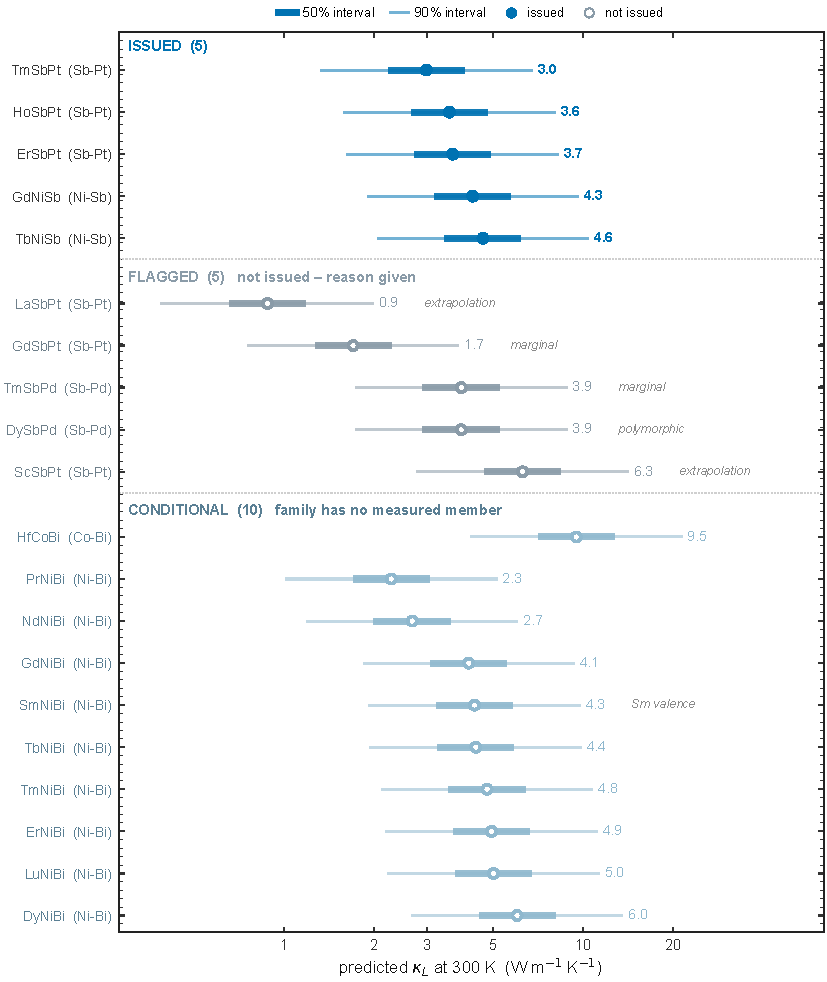
\includegraphics[width=\linewidth]{figures/fig06_landscape.pdf}
  \caption{\textbf{Everything the method can say, and what each statement is worth.} Four tiers,
  ordered by the evidence behind them: \textsc{issued}, the five predictions of
  Table~\ref{tab:predictions}; \textsc{flagged}, five compounds that clear the family test but fail
  one further check; \textsc{conditional}, ten that pass every structural and chemical screen but
  sit in a family with no usable measured anchor; and \textsc{refused}, six declined outright and
  deliberately \emph{not} plotted, since for them the calibrated value is not a quantity we are
  willing to give and drawing it with an interval would assert the opposite. Bars are the
  \SI{50}{\percent} and \SI{90}{\percent} conformal intervals; only the issued tier carries a
  filled prediction marker.}
  \label{fig:landscape}
\end{figure*}

Auditing those candidates surfaced a check we had not been applying anywhere, and it bears on the
predictions we issue as much as on the ones we withhold. Where a compound has been calculated by
more than one group the published values need not agree: across the \num{151} half Heuslers with
two or more independent transport calculations at \SI{300}{\kelvin} the median disagreement is a
factor of \num{1.13}, but the tail reaches \num{18.35}. Two candidates fail on it, and taking the
first available row for one of them, \ce{TiNiPb}, would have issued a prediction of
\SI{55.6}{\watt\per\meter\per\kelvin}---nearly three times the highest value ever measured for any
half Heusler. Independent groups also place the \ce{ErSbPt} and \ce{HoSbPt} calculations \num{1.68}
and \num{1.72} apart; the value we calibrate is mid-range in both cases, but our conformal interval
describes the error of the transfer function and not the spread among its inputs, so for those two
the stated \SI{90}{\percent} band is a lower bound on the true uncertainty.

Separately, we screened compounds with a known crystal structure but no published lattice thermal
conductivity of any kind. One survives: \ce{GaCoMo}, predicted at
\SI{11.3}{\watt\per\meter\per\kelvin} at \SI{300}{\kelvin} (\SI{90}{\percent} interval
\SIrange{5.0}{25.3}{}). Having no published calculation, it must first have one supplied by the
regression model and only then calibrated, so it carries two errors in series by the composite route
that Section~\ref{sec:deployed} shows to be the less accurate. With a chemistry supported by only
three training compounds, we present it as a screening-grade statement---that its conductivity is of
order \SI{10}{\watt\per\meter\per\kelvin} rather than \num{1} or \num{100}---and not as a prediction
on the footing of Table~\ref{tab:predictions}.

\subsection{Limits of the method}
\label{sec:limitations}

Four limitations bound what has been shown beyond those already stated above, and each carries the
number that quantifies it. The first three are recorded where they arise: the temperature slope is
not predicted (Section~\ref{sec:blind}), the family error is an interpolation figure rather than an
extrapolation test (Section~\ref{sec:failure}), and the separation from the nulls sits at the
conventional threshold and does not survive dropping the domain screens
(Section~\ref{sec:vsnulls}). Two quantities complete the first of those: across the \num{33}
in-domain compounds with at least four measured temperatures spanning a factor of \num{1.5} in $T$,
the measured logarithmic slope $\mathrm{d}\ln\kappa_L/\mathrm{d}\ln T$ spans \numrange{-4.78}{0.76}
while the predicted slope spans only \numrange{-0.74}{0.13}, and the rank correlation between them
is $\rho=-\num{0.34}$ ($p=\num{0.05}$)---not merely absent but weakly negative. Compounds governed
by a mechanism with a distinctive temperature signature---bipolar conduction at high
temperature~\cite{li2015synthesis}, or resonant rattling modes~\cite{jana2016the}---are not
distinguished from ordinary ones by anything in our model.

\textbf{The correction is empirical, not a measurement of microstructure.} Its temperature
dependence resembles boundary-limited transport in the Callaway sense~\cite{callaway1959model},
which is why the form was chosen, but the Cauchy--Schwarz argument of
Section~\ref{sec:transfer} caps the log-slope of any single-boundary-length model at $1-c=\num{0.49}$
while our fitted $p=\num{0.80}$ exceeds that ceiling by a factor of \num{1.63}: a quantity that
violates the bound cannot be the boundary term it resembles. The transfer function therefore
absorbs point-defect scattering, site disorder, porosity and interface resistance together with any
boundary contribution. Taken literally its parameters imply a phonon boundary length of order
\SI{44}{\nano\meter}; we report that as a description of the fit, not as a microstructural
measurement, and we make no claim about the grain sizes of the reference specimens.

\textbf{Twelve compounds require the conductivity to be scaled up.} The correction is capped at
unity, encoding the statement that extrinsic scattering cannot raise conductivity above the
perfect-crystal value. Yet for \num{12} of the \num{38} in-domain compounds (\SI{32}{\percent}) the
calculation lies \emph{below} the measurement, with raw ratios as low as \num{0.33}; for those the
functional form cannot help and the residual error is irreducible within this formulation. The cases
concentrate at high temperature---the fraction of matched rows in which the calculation falls below
the measurement rises from \SI{2.9}{\percent} between \SIrange{200}{300}{\kelvin} to
\SI{44.9}{\percent} above \SI{900}{\kelvin}---and two families of explanation fit that pattern
without our being able to separate them. On the calculation side a neglected four-phonon channel
would bite hardest at high temperature and matters in half Heuslers
specifically~\cite{li2024multiphono}, though the dominant approximation in published three-phonon
calculations acts in the opposite direction~\cite{feng2017fourphonon}. On the measurement side,
radiative heat loss inflates laser-flash diffusivity at high temperature~\cite{nishi2020effect} and
bipolar conduction is not removed by a single-parabolic-band Lorenz number~\cite{kim2015characteri}.
We report the pattern rather than assign a cause, and note that it is a property of the reference
data as much as of the method.

\textbf{The calibration is a fitted quantity, not a constant.} Across refits during this work, as
the reference set changed by small amounts, $c$ moved over \numrange{0.37}{0.57}. Any application of
Eq.~\eqref{eq:transfer} to a different compound set should refit rather than adopt our values, and
any comparison with our numbers should carry that range.

\textbf{The reference data carry their own uncertainty.} The measurements against which everything
here is scored are themselves uncertain. Across \num{8545} pairs of independent measurements of the
same compound at the same temperature in our corpus, the median disagreement between laboratories is
a factor of \num{1.33} and the ninetieth percentile a factor of \num{2.00}. A method reporting
\SI{33.7}{\percent} median error is therefore operating near the reproducibility floor of the
field---a \SI{32.5}{\percent} median disagreement between laboratories against our
\SI{33.7}{\percent}---rather than comfortably above it. This is context rather than excuse: it bounds
what any method can demonstrate against this corpus, and it is a further reason to prefer the
rank-ordering claim over the absolute-accuracy one. Twenty-seven of the \num{52} measured compounds
rest on a single publication, so for half the corpus the inter-laboratory spread cannot be assessed
at all.
